\documentclass{beamer}
\usepackage{amsmath}
\usepackage{tabularx}
\usepackage{graphicx}
\usepackage{subcaption}
\usepackage{tikz}
\usetikzlibrary{arrows.meta,automata,quotes,positioning,babel}
\usetikzlibrary{shapes.geometric, arrows}
\usepackage{hyperref}
\usepackage{float}

\title{Deep Learning Approach to Link Weight Prediction}
\author{Yuchen~Hou\inst{1} \and Lawrence~Holder\inst{1}}
\institute{
	\inst{1}
	School of Electrical Engineering and Computer Science\\
	Washington State University, Pullman, WA 99164
}

\begin{document}

\frame{\titlepage}

\begin{frame}{Introduction: deep learning in different application domains}
%	\begin{itemize}[<+->]
	\begin{itemize}
		\item Image recognition
		\item Speech recognition
		\item Natural language processing
		\item Graph mining
	\end{itemize}
	\begin{figure}[H]
		\centering
		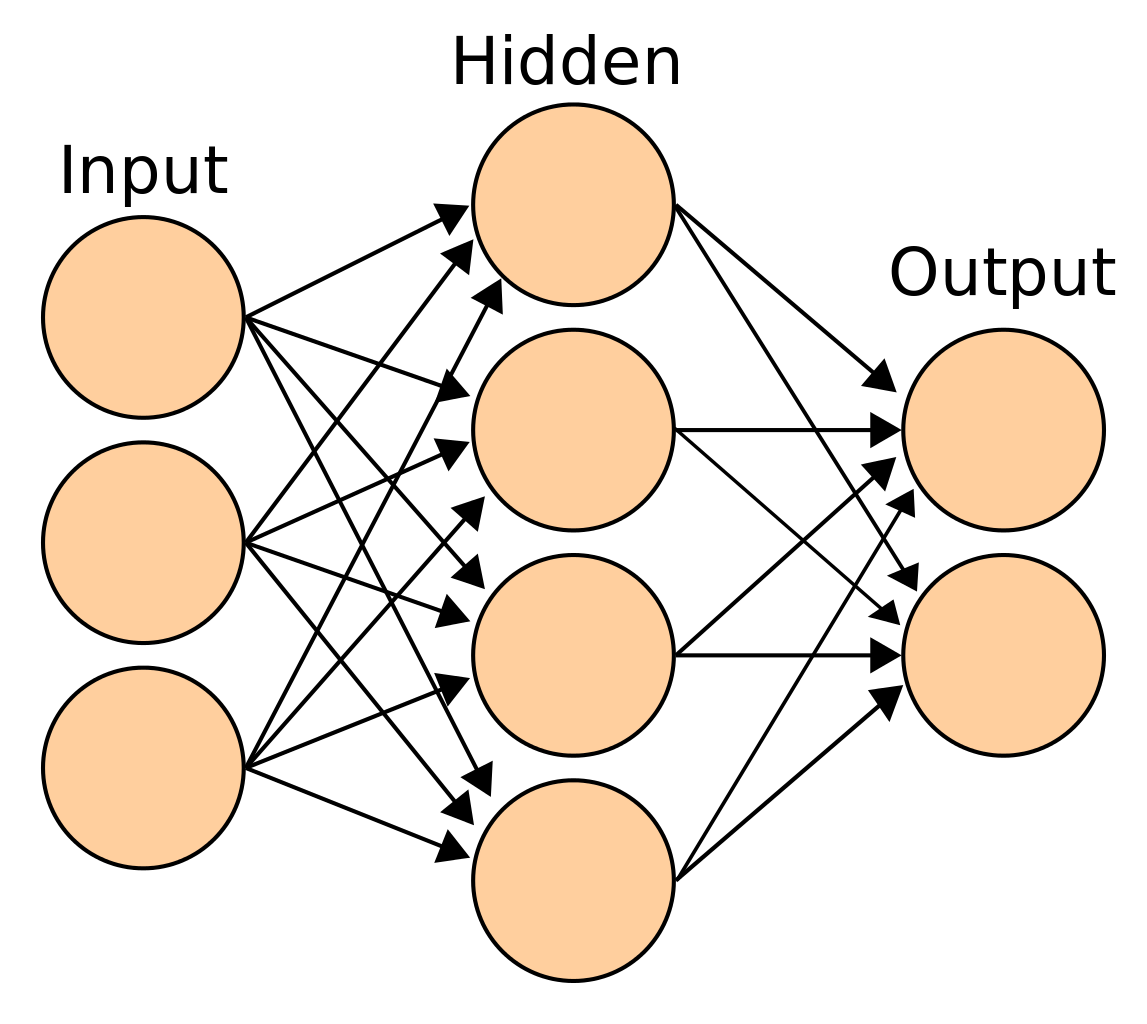
\includegraphics[width=0.5\linewidth]{ann}
		\caption{ \href{https://en.wikipedia.org/wiki/File:Artificial_neural_network.svg}{Artificial neural network} (Colin Burnett / Wikimedia Commons / Attribution-Share Alike 3.0 Unported)}
		\label{fig:neural}
	\end{figure}
\end{frame}

\begin{frame}{Background: graph mining problems}
	\begin{figure}[H]
		\centering
		\begin{subfigure}{0.49\textwidth}
			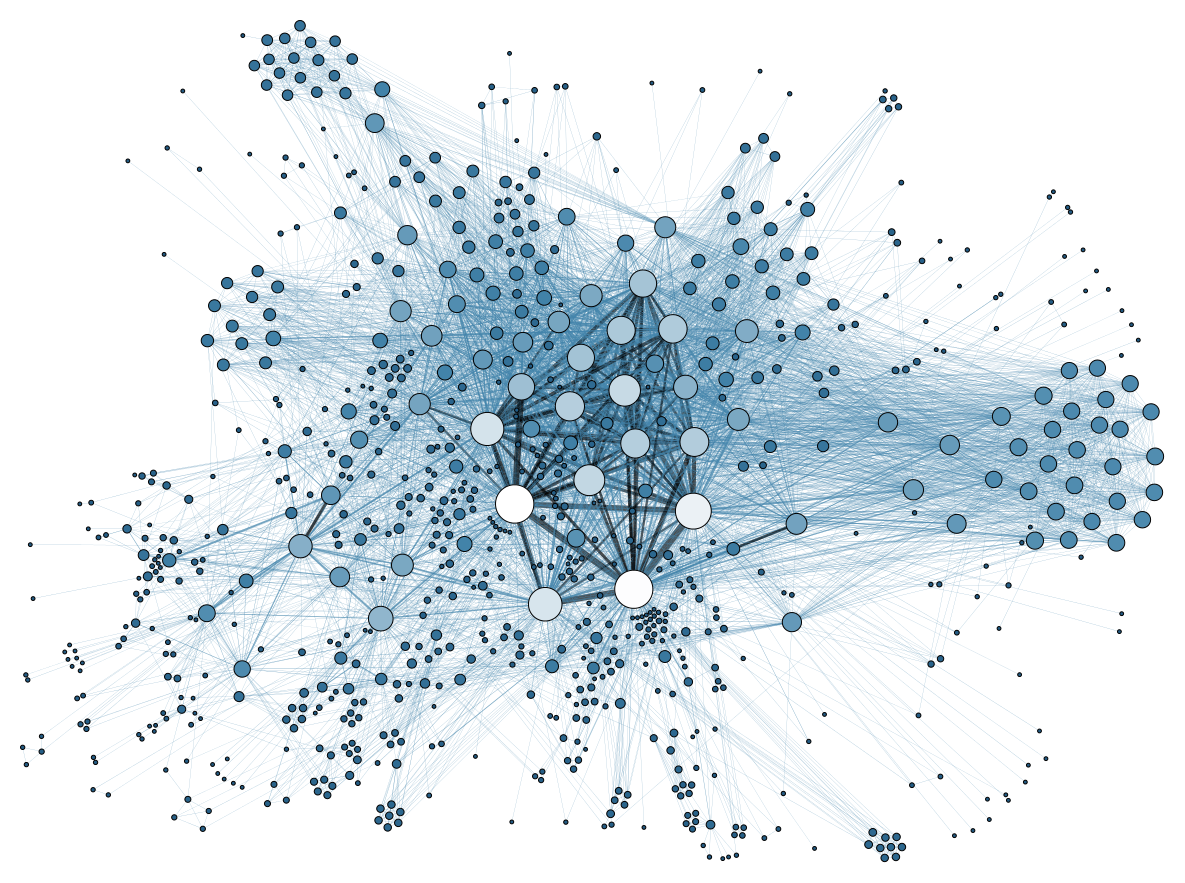
\includegraphics[width=\linewidth]{Social_Network_Analysis_Visualization}
			\caption{
				\href{https://commons.wikimedia.org/wiki/File:Social_Network_Analysis_Visualization.png}{Link prediction: predicting user connectivities in a social network} (Martin Grandjean / Wikimedia Commons / Attribution-Share Alike 3.0 Unported).
			}
			\label{fig:Social_Network_Analysis_Visualization}
		\end{subfigure}
		\begin{subfigure}{0.49\textwidth}
			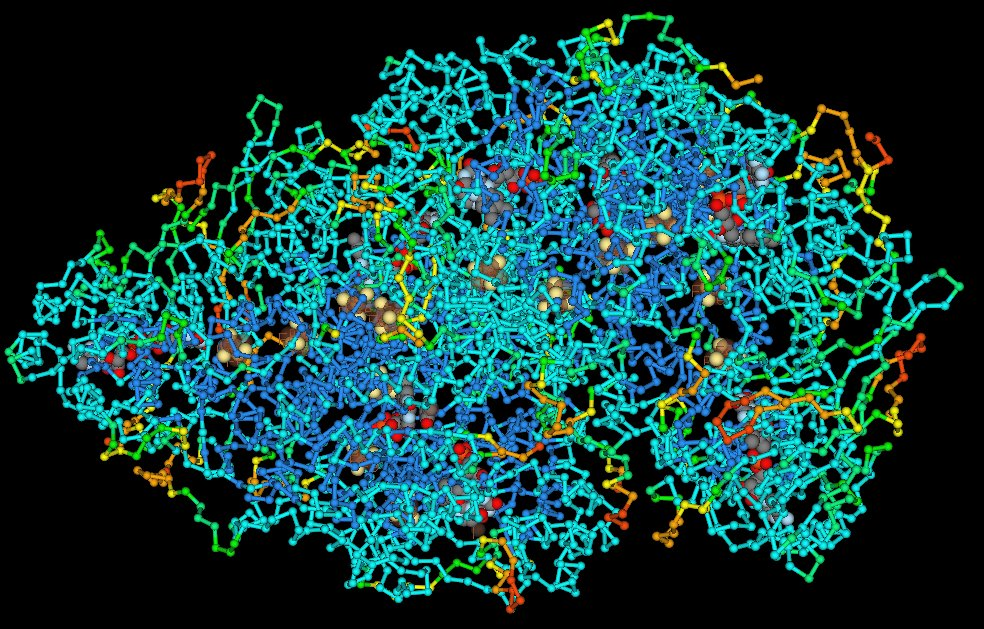
\includegraphics[width=\textwidth]{ProteinStructure}
			\caption{
				\href{https://commons.wikimedia.org/wiki/File:ProteinStructure.jpg}
				{Graph classification: predicting the chemical activity of a macromolecule} (Maksim / Wikimedia Commons / public domain).
			}
			\label{fig:protein}
		\end{subfigure}
		\caption{
			Example graph mining problems and their application scenarios.
		}
		\label{fig:trainnig}
	\end{figure}
\end{frame}

\begin{frame}{Problem: link weight prediction}{Problem example}
	\begin{figure}[H]\centering
		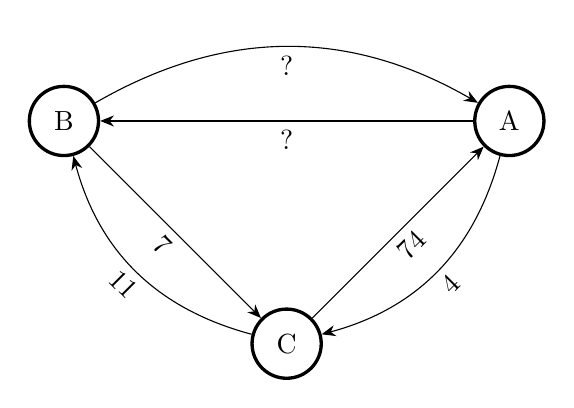
\begin{tikzpicture}[
		node distance = 4cm,
		on grid,
		> = {Stealth[length=5pt,width=4pt]},
		every state/.style = {very thick},
		every edge quotes/.style = {sloped, anchor=north}
		]
		\node[state] (B) {B};
		\node[state] (C) [below right=of B] {C};
		\node[state] (A) [above right=of C] {A};
		\path[->]   
		(A) edge["?"]   (B)
		(B) edge["7"]   (C)
		(C) edge["74"]  (A)
		(B) edge[bend left,"?"]   (A)
		(A) edge[bend left,"4"]   (C)
		(C) edge[bend left,"11"]  (B);
		\end{tikzpicture}
		\caption{
			An example of link weight prediction in a weighted directed graph -
			message volume prediction in a social network for friend recommendation.
		}
		\label{fig:example}
	\end{figure}
\end{frame}

\begin{frame}{Problem: link weight prediction}{Problem example}
	\begin{table}[H]\centering
		\caption{The edge list representation of the previous example.}
		\begin{tabularx}{\textwidth}{|X|X|X|}  \hline
			Source node & Destination node & Link weight \\ \hline
			A & B & ? \\ \hline
			A & C & 74 \\ \hline
			B & A & ? \\ \hline
			B & C & 7 \\ \hline
			C & A & 4 \\ \hline
			C & B & 11 \\ \hline
		\end{tabularx}
		\label{tab:example}
	\end{table}
\end{frame}

\begin{frame}{Problem: link weight prediction}{Problem definition}
	\begin{itemize}
		\item Given a weighted directed graph with the node set V and a link subset E
		\item Build a model weight = f(source, destination) to predict the weight of any link (source, destination) $ \notin $ E
	\end{itemize}
\end{frame}

\begin{frame}{Existing approach: pWSBM (pure Weighted Stochastic Block Model)}
	\begin{itemize}
		\item Partition the nodes in the graph into node groups
		\item Each group consists of topologically similar nodes
		\item Connect groups by bundles to represent the original graph
		\item Each bundle weight follows a normal distribution
		\item Each link weight is an example of the bundle weight
	\end{itemize}
	\begin{figure}[H]
		\centering
		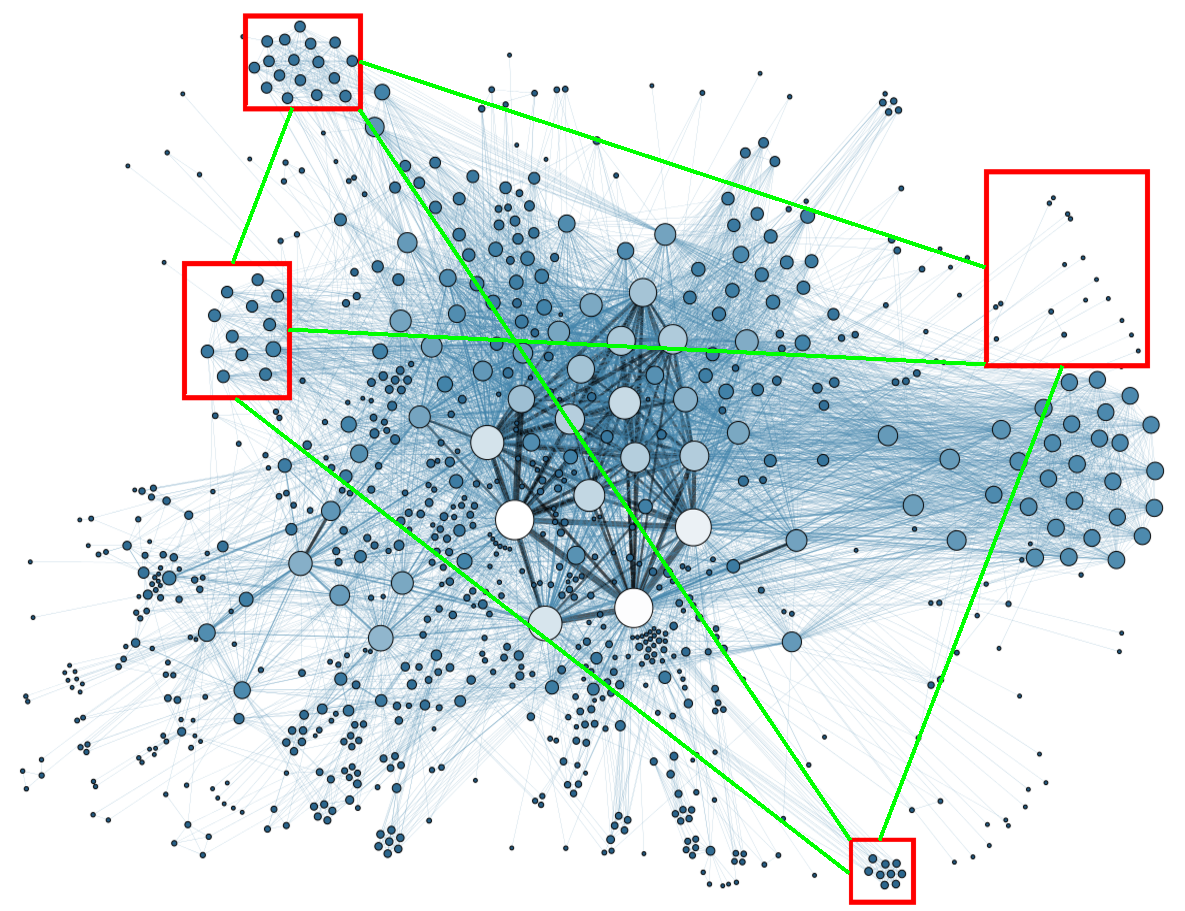
\includegraphics[width=0.4\linewidth]{SBM}
		\caption{ \href{https://commons.wikimedia.org/wiki/File:Social_Network_Analysis_Visualization.png}{pWSBM approach to link weight prediction} (Martin Grandjean / Wikimedia Commons / Attribution-Share Alike 3.0 Unported)}
		\label{fig:SBM}
	\end{figure}
\end{frame}

\begin{frame}{Motivating approach: Skip-gram model}
	\begin{itemize}
		\item word2vec: map words in sentences to vectors
		\item item2vec: reduce orders (lists of items) to sentences
		\item node2vec: reduce paths (lists of nodes) to sentences
	\end{itemize}
	\begin{figure}[H]
		\centering
		\newcommand{\layersep}{2cm}
		\newcommand{\vocabularySize}{4}
		\newcommand{\embeddingSize}{2}
		\begin{tikzpicture}[shorten >=1pt,->,draw=black!50, node distance=\layersep]
		\tikzstyle{every pin edge}=[<-,shorten <=1pt]
		\tikzstyle{neuron}=[circle,fill=black!25,minimum size=16pt,inner sep=0pt]
		\tikzstyle{input neuron}=[neuron, fill=green!50];
		\tikzstyle{output neuron}=[neuron, fill=red!50];
		\tikzstyle{hidden neuron}=[neuron, fill=blue!50];
		\tikzstyle{annot} = [text width=4em, text centered]
		
		% Draw the input layer
		\foreach \name / \y in {1,...,\vocabularySize}
		% This is the same as writing \foreach \name / \y in {1/1,2/2,3/3,4/4}
		\node[input neuron, pin=left:$ w_\y $] (I-\name) at (0,-\y) {};
		
		% Draw the hidden layer
		\foreach \name / \y in {1,...,\embeddingSize}
		\path[yshift=-1cm]
		node[hidden neuron] (H-\name) at (\layersep,-\y cm) {};
		
		% Draw the output layer
		\foreach \name / \y in {1,...,\vocabularySize}
		\node[output neuron, pin={[pin edge={->}]right:$ w_\y $}] (O-\name) at (2*\layersep,-\y) {};
		
		% Connect the input layer with the hidden layer
		\foreach \source in {1,...,\vocabularySize}
		\foreach \dest in {1,...,\embeddingSize}
		\path (I-\source) edge (H-\dest);
		
		% Connect the hidden layer with the output layer
		\foreach \source in {1,...,\embeddingSize}
		\foreach \dest in {1,...,\vocabularySize}
		\path (H-\source) edge (O-\dest);
		
		% Annotate the layers
		\node[annot,above of=H-2] {embedding layer};
		\node[annot,above of=I-2] {input layer};
		\node[annot,above of=O-2] {output layer};
		\end{tikzpicture}	
		\caption{The skip-gram model with vocabulary size 4 and embedding size 2.}
		\label{fig:skipGram}
	\end{figure}
\end{frame}

\begin{frame}{Deep learning approach: Model R}
	\begin{figure}[H]
		\centering
		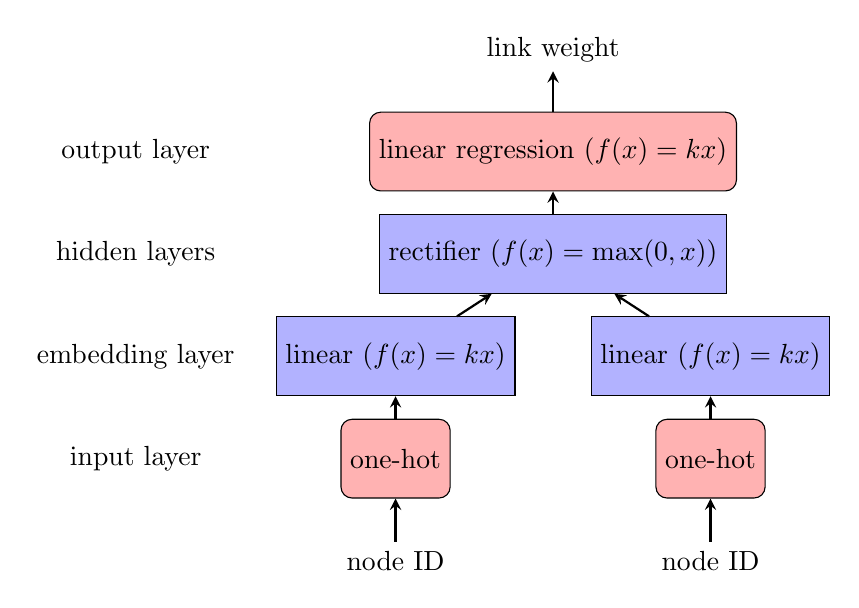
\begin{tikzpicture}[node distance=1.3cm]
		\tikzstyle{startstop} = [rectangle, rounded corners, minimum width=1cm, 
		minimum height=1cm, text centered, draw=black, fill=red!30]
		\tikzstyle{process} = [rectangle, minimum width=1cm, minimum height=1cm, 
		text centered, draw=black, fill=blue!30]
		\tikzstyle{arrow} = [thick,->,>=stealth]
		\node (linearRegression) [startstop] {linear regression ($ f(x) = kx $)};
		\node (relu) [process, below of=linearRegression] {rectifier ($ f(x) = \max (0, x) $)};
		\node (linear1) [process, below of=relu, xshift=-2cm] {linear ($ f(x) = kx $)};
		\node (linear2) [process, below of=relu, xshift=2cm] {linear ($ f(x) = kx $)};
		\node (oneHot1) [startstop, below of=linear1] {one-hot};
		\node (oneHot2) [startstop, below of=linear2] {one-hot};
		\node (weight) [above of=linearRegression] {link weight};
		\node (output) [left of=linearRegression, xshift=-4cm] {output layer};
		\node (hidden) [below of=output] {hidden layers};
		\node (embedding) [below of=hidden] {embedding layer};
		\node (input) [below of=embedding] {input layer};
		\node (source) [below of=oneHot1] {node ID};
		\node (destination) [below of=oneHot2] {node ID};
		\draw [arrow] (source) -- (oneHot1);
		\draw [arrow] (destination) -- (oneHot2);
		\draw [arrow] (oneHot1) -- (linear1);
		\draw [arrow] (oneHot2) -- (linear2);
		\draw [arrow] (linear1) -- (relu);
		\draw [arrow] (linear2) -- (relu);
		\draw [arrow] (relu) -- (linearRegression);
		\draw [arrow] (linearRegression) -- (weight);
		\end{tikzpicture}
		\caption{The Model R (R as in "relation") for link weight prediction.}
		\label{fig:model}
	\end{figure}
\end{frame}

\begin{frame}{Comparison: pWSBM vs Model R}
	\begin{table}[H]\centering
		\caption{Model R has advantages over pWSBM in several aspects.}
		\begin{tabularx}{\textwidth}{|X|c|c|}  \hline
			Aspect & pWSBM & Model R \\ \hline
			model granularity & node group level & node level \\ \hline
			distribution assumption & normal distribution & NA \\ \hline
			model flexibility & low & high \\ \hline
		\end{tabularx}
		\label{tab:comparison}
	\end{table}
\end{frame}

\begin{frame}{Experiments}{Learning techniques}
	\begin{itemize}
		\item Backpropagation
		\item Stochastic gradient descent
		\item Mini-batch
		\item Early stopping
	\end{itemize}	
\end{frame}

\begin{frame}{Experiments}{Baseline approaches}
	\begin{itemize}
		\item SBM (Stochastic Block Model)
		\item pWSBM (pure Weighted Stochastic Block Model)
		\item bWSBM (balanced Weighted Stochastic Block Model)
		\item DCWBM (Degree Corrected Weighted Stochastic Block Model)
	\end{itemize}
\end{frame}

\begin{frame}{Experiments}{Datasets}
	\begin{table}[H]\centering
		\caption{The datasets used in experiments.}
		\begin{tabularx}{\textwidth}{|X|c|c|}  \hline
			Dataset & Nodes & Link weight semantics \\ \hline
			Airport & 500 airports & number of passengers delivered \\ \hline
			Collaboration & 226 nations & number of papers coauthored \\ \hline
			Congress & 163 committees  & number of members shared \\ \hline
			Forum  & 1899 users & number of messages sent \\ \hline
		\end{tabularx}
		\label{tab:datasets}
	\end{table}
\end{frame}

\begin{frame}{Experiments}{Results}
	\begin{figure}[H]\centering
		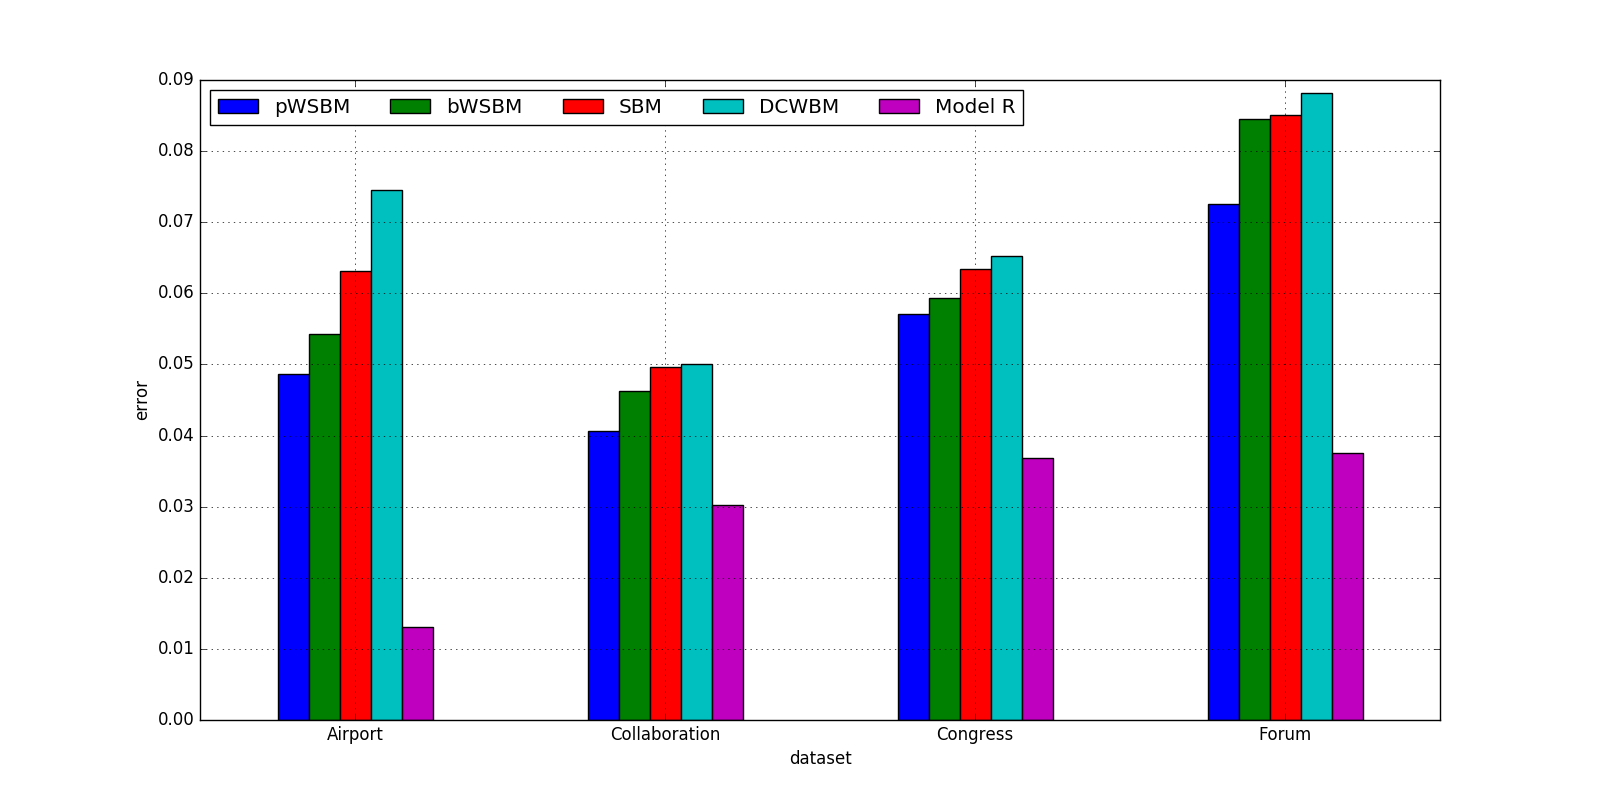
\includegraphics[width=\textwidth]{link-weight-errors}
		\caption{
			Model R has the lower mean squared errors than 4 baseline approaches over 5 datasets consistently.
		}
		\label{fig:errors}
	\end{figure}
\end{frame}

\begin{frame}{Conclusions}
	\begin{itemize}
		\item Model R uses node vectors to predict unknown link weights
		\item Model R is more accurate than Stochastic Block Model based approaches
		\item Deep learning can be successfully applied to link weight prediction problem
	\end{itemize}
\end{frame}

\begin{frame}{Future work}
	\begin{itemize}
		\item Node embedding semantics
		\item Unified embedding space for source and destination nodes
	\end{itemize}
\end{frame}

\end{document}